\documentclass[final,xcolor=svgnames,A4]{beamer}
\usepackage[english]{babel}
\usepackage[T1]{fontenc}
\usepackage[utf8]{inputenc}
\usepackage{microtype}
\usepackage[noend]{algpseudocode}
\newcommand*\Let[2]{\State #1 $\gets$ #2}
\usetheme{default}
\setbeamercovered{invisible}
\useoutertheme{infolines}
\usepackage{eso-pic}
% \usepackage{monster2e}
\usepackage{tikz}
\usepackage{layout}
\usepackage{xcolor}
\usepackage{amsmath,amssymb}
\usepackage{fancybox}
\usepackage{graphicx}
\usepackage[absolute,showboxes,overlay]{textpos}
\TPshowboxesfalse
\textblockorigin{0mm}{0mm}
\usepackage{appendixnumberbeamer}

\setbeamertemplate{navigation symbols}{}

\renewcommand{\sfdefault}{lmss}
\sffamily

\setbeamersize{text margin left=1cm,text margin right=1cm}

\setlength{\parindent}{0pt}
\setlength{\parskip}{6pt plus 2pt minus 1pt}
\setlength{\emergencystretch}{3em}  % prevent overfull lines
\setcounter{secnumdepth}{0}
\newcommand{\pcc}{\textsc{Correlation Clustering}}
\usepackage[citestyle=authoryear-comp,bibstyle=ieee,isbn=false,maxnames=1,minnames=1,sorting=nyt,backend=biber,defernumbers=true]{biblatex}

\AtEveryBibitem{
   \clearfield{arxivId}
   % \clearfield{booktitle}
   \clearfield{doi}
   \clearfield{eprint}
   \clearfield{eventdate}
   \clearfield{isbn}
   \clearfield{issn}
   % \clearfield{journaltitle}
   \clearfield{month}
   % \clearfield{number}
   \clearfield{pages}
   \clearfield{series}
   \clearfield{url}
   \clearfield{urldate}
   \clearfield{venue}
   % \clearfield{volume}
   \clearlist{location} % alias to field 'address'
   \clearlist{publisher}
   \clearname{editor}
}
\addbibresource{../../../biblio/magnet.bib}

% \title{Correlation Clustering}
% \author{Géraud Le Falher --- MAGNET}
% \date{January 22, 2015}
\renewcommand{\theauthor}{Géraud Le Falher}
\newcommand{\shorttitle}{Signed graphs: clustering and link prediction}
\newcommand{\mydate}{January 22, 2015}

\begin{document}

\setbeamertemplate{background canvas}{\includegraphics[width=\paperwidth,height=\paperheight]{fond_inria}} 
\setbeamertemplate{footline}{ \hspace{5em} \raisebox{2em}{\textcolor{white}%
	{\large \theauthor{} --- MAGNET\hspace{5em}\mydate{}}}\hspace{2em} }

\begin{frame}

\begin{textblock*}{7cm}(13mm,50mm)
	{\textcolor{white} {
			{\huge \shorttitle{}}
		}
	}
	\end{textblock*}

\vspace*{-4pt}
\end{frame}
\setbeamertemplate{background canvas}{\includegraphics[width=\paperwidth,height=\paperheight]{fond_bas}} 
\setbeamertemplate{footline}{
\hspace{2cm} 
\raisebox{2.0ex}
{\textcolor{white}{\theauthor{} --- \shorttitle{}}}\hfill 
  \raisebox{2.0ex}
  {\textcolor{white}{\insertframenumber~/~\inserttotalframenumber \hspace{1em}}}}


\begin{frame}{Outline}
\tableofcontents
\end{frame}

\begin{frame}{Applications}
	\section{Applications}
	A major source of signed graphs are graphs of social interactions, in
	which we want to:
		\begin{itemize}
			\item find antagonistic groups in signed graphs or in users/items
				bipartite graphs (Youtube, Amazon, etc) \autocite{Bipartite12}
			\item predict sign of unknown links \autocite{Leskovec2010}, for
				instance to improve recommendation relevance
		\end{itemize}
\end{frame}

\begin{frame}
	\begin{figure}[h]
		\centering
		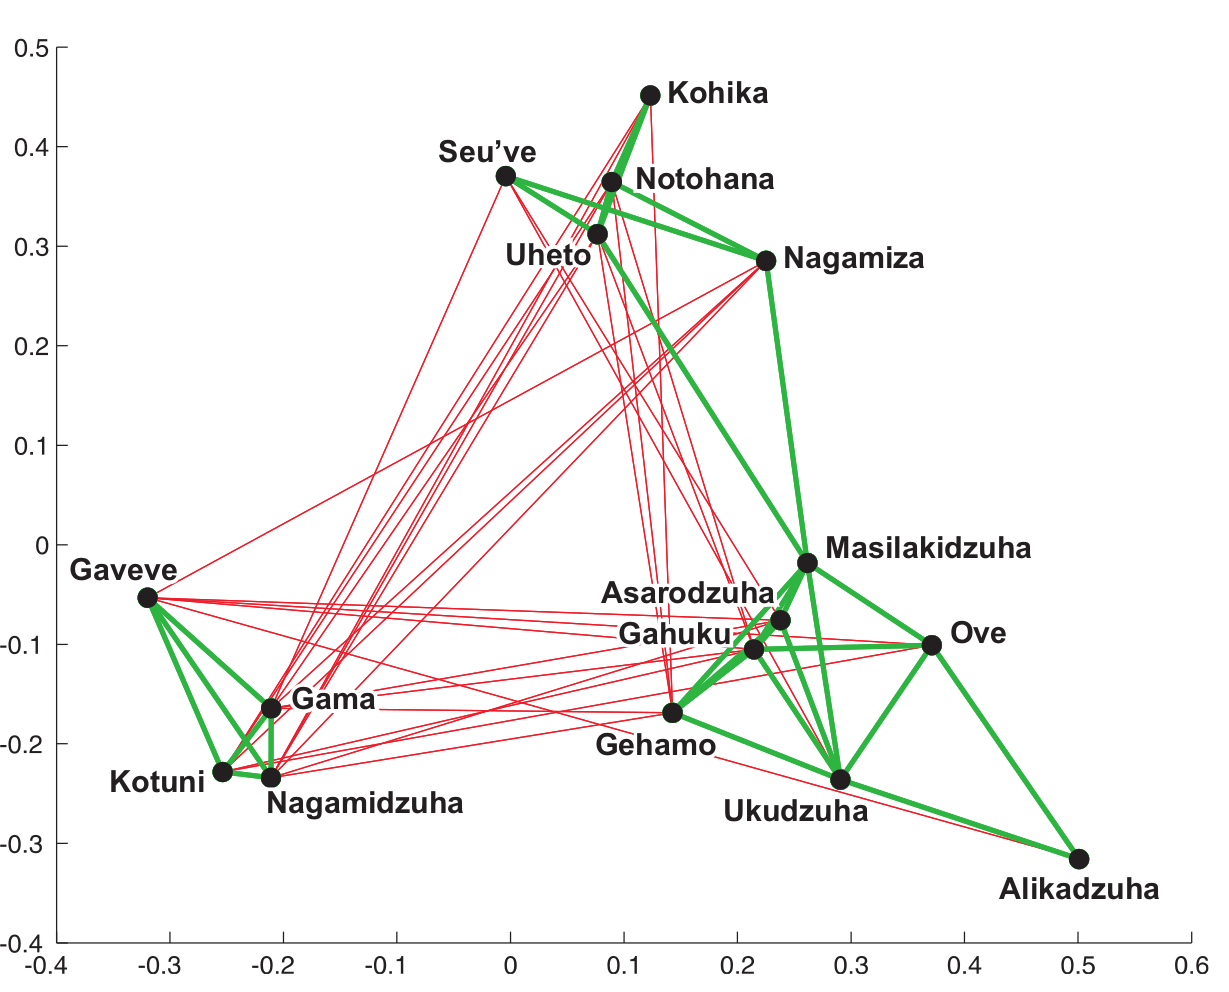
\includegraphics[width=0.75\linewidth]{tribes.png}
		\caption{Friendly and antagonistic relations between 16 New Guinean
			tribes, belonging to three higher order groups found by
			ethnological observations \autocite{Luca10}}
	\end{figure}
\end{frame}

\begin{frame}
	\begin{figure}[h]
		\centering
		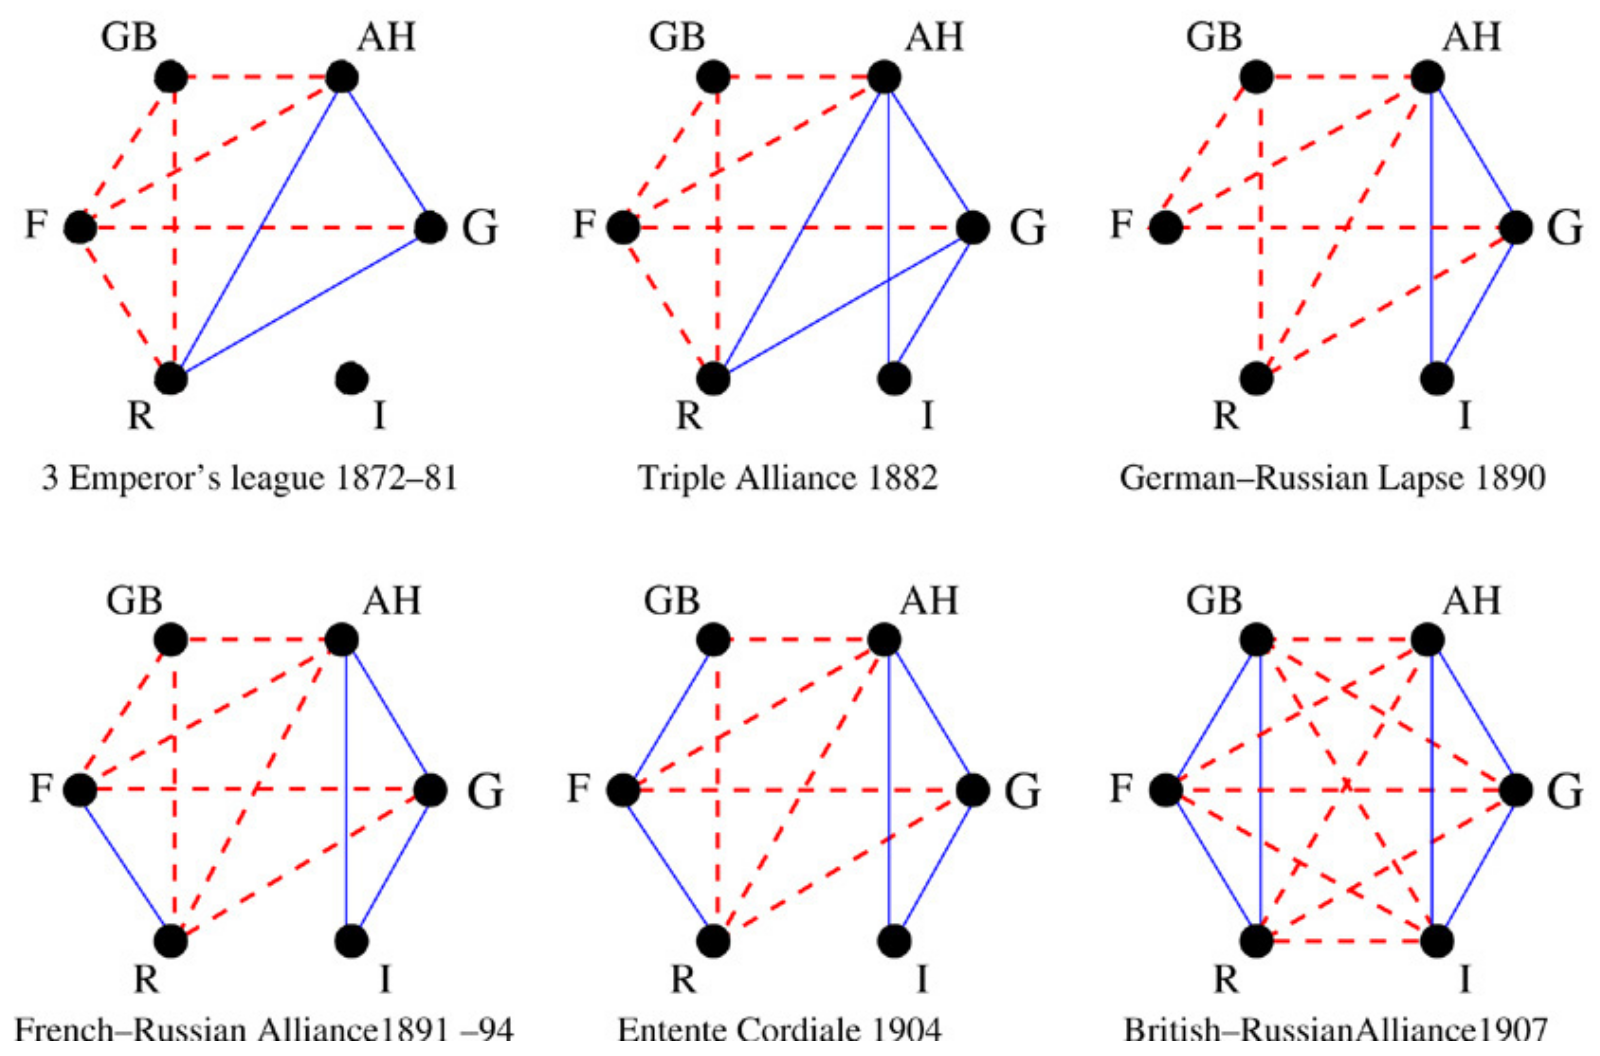
\includegraphics[width=0.8\linewidth]{europe.png}
		\caption{Military alliances between European states before WW1 \autocite{Antal2006a}}
	\end{figure}
\end{frame}

\begin{frame}
	\begin{figure}[h]
		\centering
		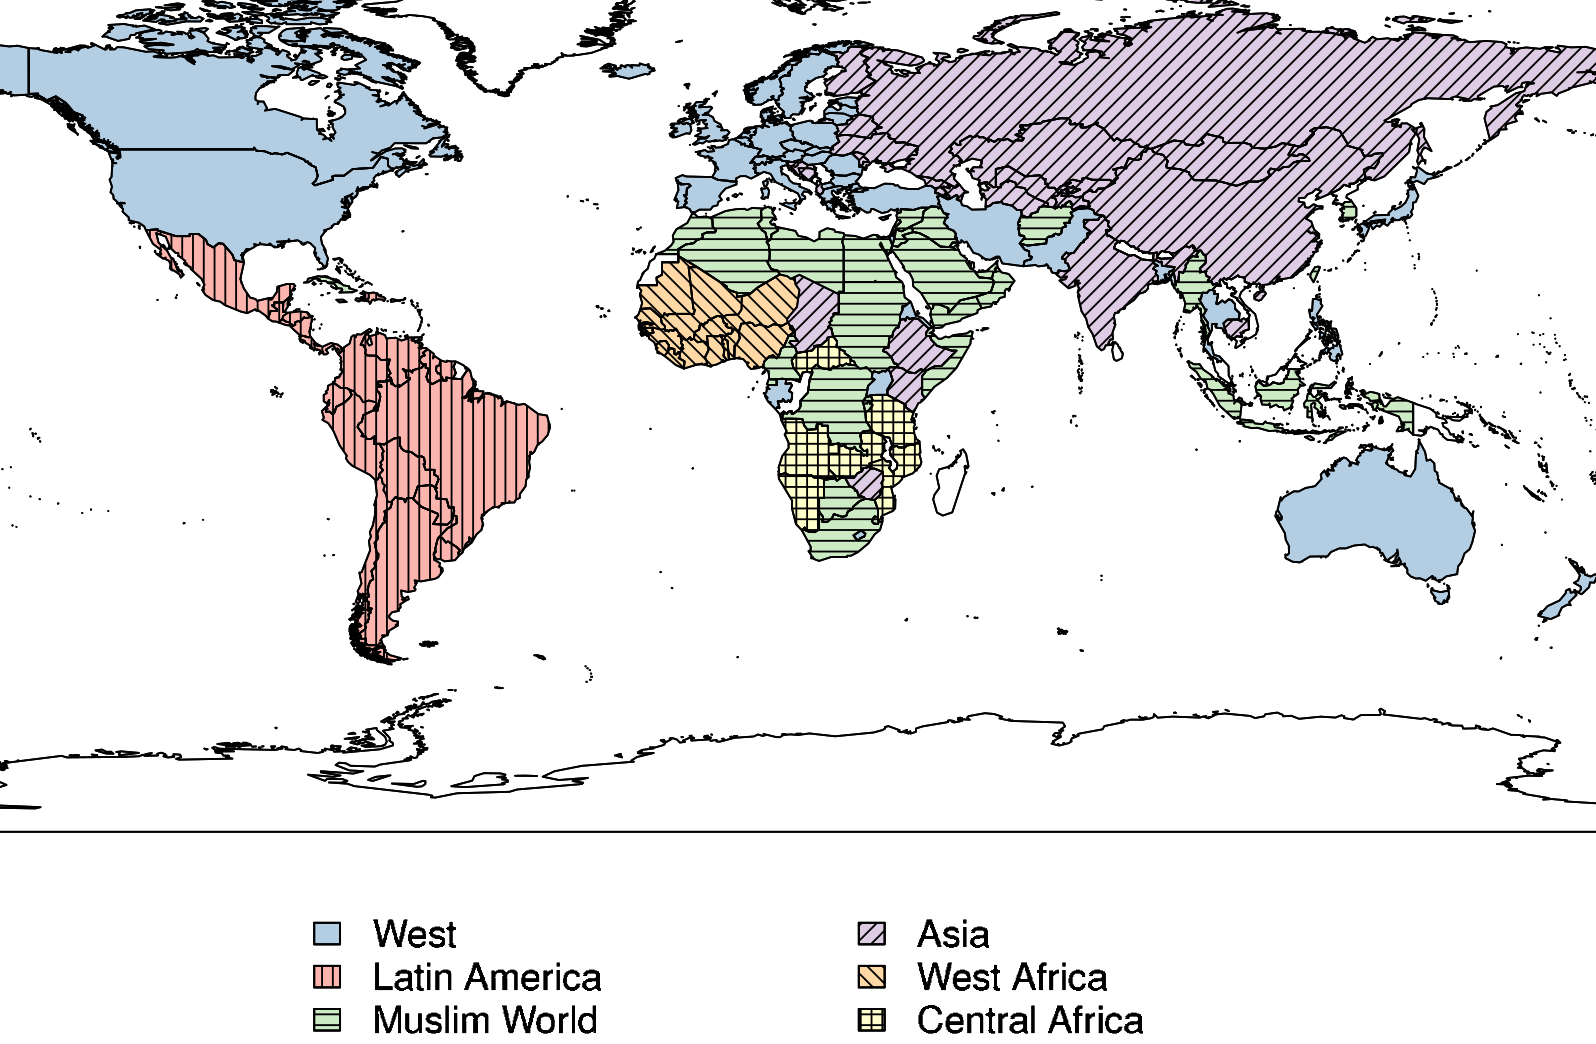
\includegraphics[width=0.8\linewidth]{world.png}
		\caption{Correlates of war between 1993 and 2001, somehow reflect
			Huntington blocks \autocite{Traag2009}}
	\end{figure}
\end{frame}

\section[]{Problem}
\begin{frame}{The \pcc{} problem \autocite{Bansal2002}}

\only<1-1>{\begin{textblock*}{80mm}[0,0](45mm,3.6em)
\includegraphics[width=80mm]{nobjects.pdf}
\end{textblock*}}
\only<2-2>{\begin{textblock*}{80mm}[0,0](45mm,3.6em)
\includegraphics[width=80mm]{brelations.pdf}
\end{textblock*}}
\only<3-3>{\begin{textblock*}{80mm}[0,0](45mm,3.6em)
\includegraphics[width=80mm]{tclusters.pdf}
\end{textblock*}}
\only<4->{\begin{textblock*}{80mm}[0,0](45mm,3.6em)
\includegraphics[width=80mm]{edisa.pdf}
\end{textblock*}}

\uncover<1->{
\begin{block}{input}
	\vspace{-1\baselineskip}
	\begin{itemize}
		\itemsep1pt\parskip0pt\parsep0pt
		\item $n$ objects
		\uncover<2->{\item binary relation \\ between \\ (some of) them}
	\end{itemize}
\end{block}
}

\uncover<3->{
\begin{block}{output}
	\vspace{-1\baselineskip}
	clustering
\end{block}
}

\uncover<4->{
\begin{block}{measure of quality}
	\vspace{-1\baselineskip}
	\begin{itemize}
		\itemsep1pt\parskip0pt\parsep0pt
		\item Some edges are disagreeing
		\item we want to minimize their number
	\end{itemize}
\end{block}
}

\end{frame}

\section[]{State of the art}
\begin{frame}{State of the art}
	Two main approaches, depending of the input
	\begin{columns}[t]
		\begin{column}{0.5\linewidth}
			\uncover<1->{
			\begin{block}{Complete graph}
				\begin{itemize}
					\item NP-complete by reduction from the multicut problem \autocite{Demaine2006}
					\uncover<1->{\item There is a quadratic combinatorial randomized
						approximation whose expected cost is at most 3 times
						the optimal one \autocite{Ailon2008}}
				\end{itemize}
			\end{block} 
		}
		\end{column}
		\begin{column}{0.5\linewidth}
			\uncover<2->{
			\begin{block}{General graph}
				\begin{itemize}
					\item There is a polynomial approximation (of ratio
						$O(\log n)$) that solves a large linear program \autocite{Demaine2006}.
					\uncover<2->{\item But less information so for any constant $c$,
						getting a $O(c)$ approximation is NP-Hard.}
				\end{itemize}
			\end{block}   
		}
		\end{column}
	\end{columns}  
\end{frame}

\begin{frame}{State of the art}
	% \begin{columns}[t]
	% 	\begin{column}{0.7\linewidth}
	% 		\uncover<1->{
				\begin{block}{Complete graph}
					\begin{algorithmic}[0]
						\Function{\textsc{CC-Pivot}}{$G=(V,\,E)$}
						\While{not all nodes are clustered}
							\Let{$pivot$}{pick a node in $V$ at random}
							\State put $pivot$ in its own cluster
							\State add all its positive neighbors
							\State remove them from $G$
						\EndWhile
						\EndFunction
					\end{algorithmic}
					\vspace*{3\baselineskip}
					\only<1-1>{\begin{textblock*}{55mm}[0,0](65mm,45mm)
							\includegraphics[width=55mm]{brelations.pdf}
						\end{textblock*}}
					\only<2-2>{\begin{textblock*}{55mm}[0,0](65mm,45mm)
							\includegraphics[width=55mm]{c1.pdf}
						\end{textblock*}}
					\only<3-3>{\begin{textblock*}{55mm}[0,0](65mm,45mm)
							\includegraphics[width=55mm]{c2.pdf}
						\end{textblock*}}
					\only<4->{\begin{textblock*}{55mm}[0,0](65mm,45mm)
							\includegraphics[width=55mm]{tclusters.pdf}
						\end{textblock*}}
					\uncover<5->{Solving the linear program \\ brings a $2.5$ approximation}
				\end{block}   
	% 		}
	% 	\end{column}
	% \end{columns}  
\end{frame}

\section[]{Our method (so far)}
\begin{frame}{Our method for general graph}
	\begin{block}{idea}
		\begin{itemize}
			\item complete the graph in a combinatorial fashion
			\item run \textsc{CC-Pivot}
			\item keep the clustering induced on the original graph
		\end{itemize}
		\centering
		\includegraphics[width=.7\linewidth]{triangles.pdf}
	\end{block}

	% \only<1->{\begin{textblock*}{30mm}[0,0](92mm,6mm)
			% \includegraphics[height=65mm]{triangles.pdf}
		% \end{textblock*}}
\end{frame}

\begin{frame}[t]{Ongoing work}
	\begin{block}{goals}
		\begin{itemize}
				\item reasonable polynomial complexity
				\item $O(\log n)$ approximation in the worst case
				\item better for \enquote{realistic average-case}
					\autocite{Makarychev2014}
		\end{itemize}
	\end{block}
	\begin{block}{means}
	\begin{itemize}
		\item A crucial point is how to choose the pivot for completing
		\item Experimental evaluation of several strategies
		\item Analysis on simple cases
		% \item Identification of which subclasses of graphs lead to constant or
		% 	$O(\log n)$ approximation in polynomial time
	\end{itemize}
	\end{block}
\end{frame}

\appendix
\begin{frame}[t,allowframebreaks]
	\frametitle{References}
	\printbibliography
\end{frame}

%%%%%%%%%%%%%%%%%%%%%%%%%%%
\setbeamertemplate{background canvas}{\includegraphics[width=\paperwidth,height=\paperheight]{derniere-sc-en}} 
\setbeamertemplate{footline}{}


\begin{frame}

\begin{center} 
\textcolor{white} {\huge Thank you for your attention}
\end{center}
\begin{center} 
\textcolor{white} {\Large Questions?}
\end{center} 
\end{frame}

\setbeamertemplate{background canvas}{\includegraphics[width=\paperwidth,height=\paperheight]{basrouge}} 
\begin{frame}[t]{Linear Program}
	\begin{align*}
		\min \sum_{(i,\, j)\in E^+} (1-x_{ij}) w_{ij} +
		\sum_{(i,\, j)\in E^-} x_{ij} w_{ij} \\
		x_{ij} =   \begin{cases}
			1 & \text{if $i$ and $j$ are in the same cluster} \\
			0       & \text{otherwise}
		\end{cases} \\
		x_{ij} \in [0,\,1]
	\end{align*}
\end{frame}
\end{document}

